% $Date$
\documentclass[12pt,a4paper]{article}
\usepackage[polish]{babel}                      % Język polski
\usepackage[utf8]{inputenc}                     % Kodowanie dokumentu
\usepackage[T1]{fontenc}                        % Kodowanie fontów
%\usepackage{lmodern}
\usepackage{times}                              % Font wektorowy
\usepackage[cm]{fullpage}                       % Cała szerokość strony
%\usepackage[pdftex,bookmarks,colorlinks]{hyperref} % Linki w dokumencie PDF
\usepackage[pdftex,bookmarks]{hyperref} % Linki w dokumencie PDF
\usepackage{indentfirst}                        % Wcięcia akapitów
\usepackage{graphicx}                           % Grafika w png, jpeg, gif
\usepackage{float}                              % Ulepszone rozmieszczanie
%\pagestyle{headings}
%\graphicspath{{png}}                            % Szuka grafik w katalogu png
\frenchspacing                                  % Odstępy międzyzdaniowe

\title{ConvML 1.2}
\author{Marcin Kacprzak\\ marcin.kacprzak@entertech.com.pl\\
  \and Piotr Kulinowski\\ piotr.kulinowski@entertech.com.pl}
\date{\today}

\begin{document}

\maketitle

\begin{abstract}
  Ten dokument zawiera opis funkcji i składni języka ConvML.  ConvML jest
  językiem do zapisu strukturalnego modelu przenośnika taśmowego w formacie XML
  \cite{XML10}.

  Wersję PDF tego dokumentu można odnaleźć pod adresem
  \href{http://www.entertech.com.pl/convml/convml.pdf}{entertech.com.pl/convml/convml.pdf}.

  Schema opisywanego języka znajduje się pod adresem
  \href{http://www.entertech.com.pl/convml/convml\_11.xsd}{entertech.com.pl/convml/convml\_11.xsd}.
\end{abstract}

\tableofcontents


\section{Wstęp}
Potrzeba opracowania modelu strukturalnego przenośnika taśmowego wynikła z
informatycznej konieczności wprowadzenia procedury zapisu pełnej informacji o
urządzeniu, która jednoznacznie i spójnie opisywałaby parametry
techniczno-ruchowe i konfigurację przenośnika taśmowego.  Ze względu na
uniwersalność zapisu i chęć popularyzacji modelu strukturalnego wprowadzono
anglojęzyczne nazewnictwo poszczególnych podzespołów.

Do opracowania systemu zapisu modelu strukturalnego przenośnika taśmowego
wykorzystano język XML Schema \cite{XSD0}, ułatwiający definiowanie struktury i
kolejności podzespołów przenośnika taśmowego oraz umożliwiający w łatwy sposób
jego adaptację na platformie informatycznej.  Istotną cechą modelu
strukturalnego jest praktycznie nieograniczona możliwość jego rozbudowy, bez
utraty przejrzystości struktury.  Każdy z elementów posiada grupę atrybutów
opisujących jego cechy, mogące być zarówno parametrami technicznymi jak i
ekonomicznymi.


\section{Konwencje}
Nazwa ConvML pochodzi od Conveyor Meta Language.  Typowy dokument ConvML ma
postać pliku tekstowego o rozszerzeniu xml lub convml.  Zalecane kodowanie to
UTF-8.

Dokument ConvML do zapisu informacji o strykturze przenośnika wykorzystuje
\emph{elementy}, a do zapisu właściwości używane są \emph{atrybuty} języka XML.
Elementy w języku ConvML mogą zawierać inne elementy oraz atrybuty, nie używa
się natomiast tekstu zawartego pomiędzy znacznikami do zapisu informacji o
przenośniku taśmowym.

Elementy języka ConvML należą do przestrzeni nazw:
http://www.entertech.com.pl/bcml.

\subsection{Wersjonowanie}
Od wersji 1.1 pliki ze schemą nazywane są convml\_WERSJABEZKROPKI.xsd. Numery
wersji zakończone liczbą nieparzystą oznaczają wersje rozwojowe, a zakończone
liczbą parzystą wersje stabilne.

\subsection{Nazwy elementów i atrybutów}
Nazwy elementów zapisywane są za pomocą tzw. \emph{Camel Case} oraz pierwszy znak jest
zapisywany wielką literą. Nazwy atrybutów zapisywane są również przy użyciu
\emph{Camel Case} ale zaczynają się małą literą.

\subsection{XSD}
Schemę zorganizowano według wzorca projektowego \emph{Venetian Blind} opisanego na
stronie \href{http://www.xfront.com/GlobalVersusLocal.html}{xFront}. Wyjątkiem jest
jedynie element {\tt Meta} gdzie świadomie zrezygnowano z tego wzorca.

Grupy atrybutów mają dodany do nazwy dodany sufiks {\tt AttrGroup}. Do nazwy typów
dodawany jest sufiks {\tt Type}.

\subsection{Referencje}
Wewnątrz instancji dokumentu mogą być utrzymywane relacje pomiędzy elementami
które nie znajdują się w bezpośrednim sąsiedztwie.

Przykładowo element {\tt Material} za pomocą atrybutu {\tt type} może wskazywać na
element {\tt MaterialType}, którego wartość atrybutu {\tt typeId} zgadza się z
wartością atrybutu {\tt type} elementu odwołującego się.

Do modelowania takich powiązań wykorzystano technikę \emph{key/keyref} będącą
częścią standardu XML Schema.

Więcej informacji na temat typów w języku ConvML znajduje się w rozdziale
\ref{sec:Types}.


\section{Struktura dokumentu}
Głównym elementem dokumentu jest {\tt ConvML}.  Podelementy {\tt Meta} oraz
{\tt Types} są opcjonalne. Element {\tt BeltConveyor} musi wystąpić co
najmniej raz aby dokument był poprawny.  Przykładowa instancja dokumentu może
mieć następującą postać:

\begin{verbatim}
<?xml version="1.0" encoding="utf-8"?>
<ConvML version="1.2">
  <Meta/>
  <Types/>
  <BeltConveyor/>
</ConvML>
\end{verbatim}  


\subsection{Element główny <ConvML>}

\begin{figure}[H]
  \centering
  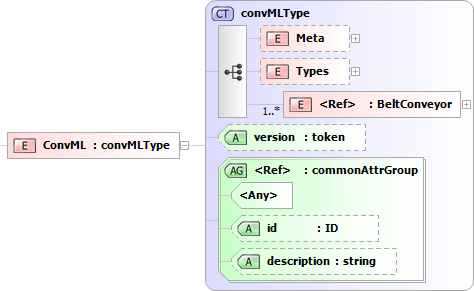
\includegraphics[width=0.6\textwidth]{png/liquid/ConvML}
  \caption{Definicja elementu ConvML}
  \label{fig:convml-xsd}
\end{figure}

\noindent\textbf{Atrybuty:}
\begin{description}
\item[version] Zastosowana w dokumencie wersja języka ConvML.
\end{description}


\subsection{Przenośnik taśmowy <BeltConveyor>}\label{sec:BeltConveyor}
Górnicze przenośniki taśmowe definiuje się jako urządzenia służące do ciągłego
transportu na taśmie materiałów sypkich, pozyskiwanych podczas procesów
związanych z prowadzeniem robót górniczych [Kulinowski2011].  Do zespołów
głównych przenośnika taśmowego należą: stacja czołowa, stacja zwrotna, stacja
napinania taśmy, taśma, trasa, zestawy krążnikowe i krążniki
\cite{Antoniak2005}.

\begin{figure}
  \centering
  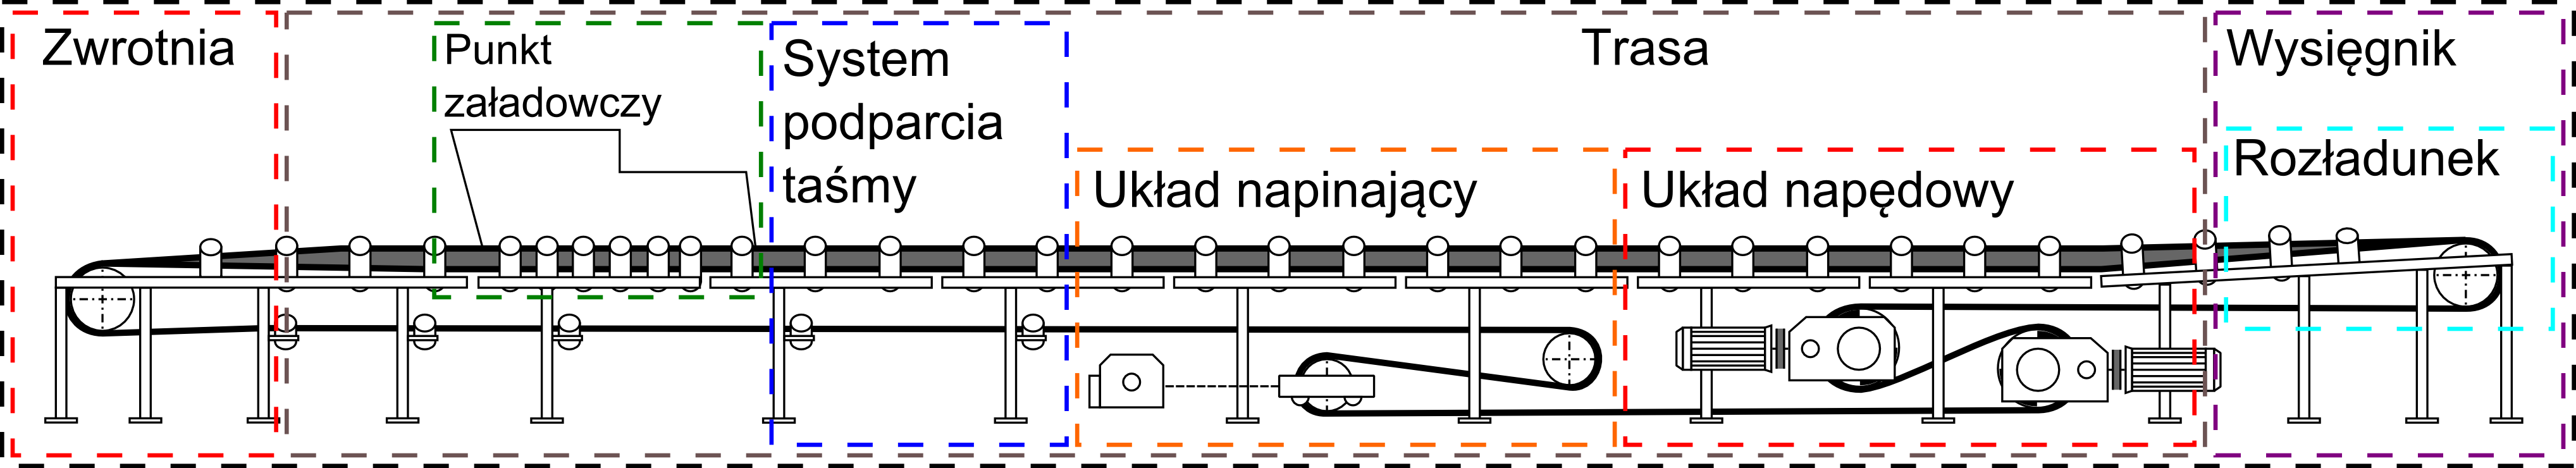
\includegraphics[width=\textwidth]{png/belt_conveyor_drw}
  \caption{Podstawowe podzespoły przenośnika taśmowego}
  \label{fig:beltConveyor-drw}
\end{figure}

W języku ConvML podstawowy podział przenośnika taśmowego wygląda następująco:

\begin{itemize}
\item Belt -- taśma,
\item Tail -- stacja zwrotna,
\item Route -- trasa,
\item Head -- stacja czołowa.
\end{itemize}

Pozostałe zespoły główne przenośnika taśmowego znajdują się głębiej w strukturze
opisywanej przez język ConvML.  System podparcia taśmy należy do elementów
składowych trasy.  Układy napędowy i napinający są powiązane z bębnami, które
mogą występować jako elementy składowe stacji zwrotnej, stacji czołowej lub
trasy.

\begin{figure}[H]
  \centering
  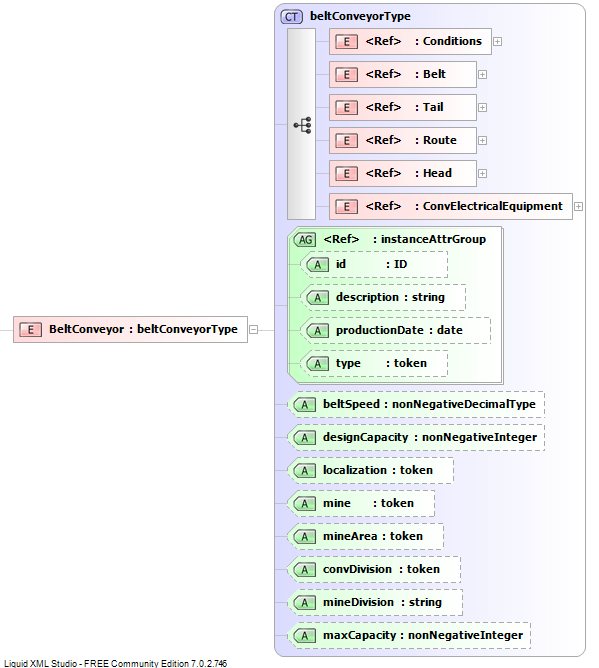
\includegraphics[width=0.6\textwidth]{png/liquid/BeltConveyor}
  \caption{Definicja elementu BeltConveyor}
  \label{fig:beltConveyor-xsd}
\end{figure}

\noindent\textbf{Rodzice:} \texttt{ConvML}

\noindent\textbf{Atrybuty:}
\begin{description}
\item[beltSpeed] Prędkość taśmy przenośnika - v [m/s]
\item[designCapacity] Wydajność nominalna przenośnika - Q [t/h]
\item[maxCapacity] Wydajność maksymalna
\end{description}


\subsection{Lokalizacja <Localization>}
Element {\tt Localization} grupuje atrybuty związane z lokalizacją przenośnika
taśmowego.

\begin{figure}[H]
  \centering
  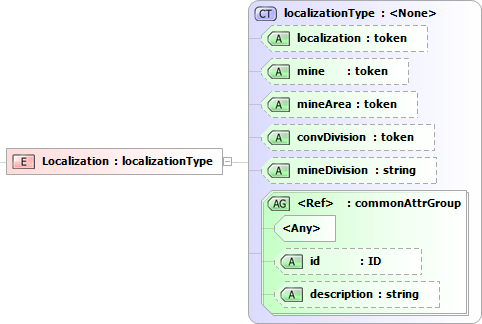
\includegraphics[width=0.6\textwidth]{png/liquid/Localization}
  \caption{Definicja elementu Localization}
  \label{fig:conditions-xsd}
\end{figure}

\noindent\textbf{Rodzice:} \texttt{ConvML}

\noindent\textbf{Atrybuty:}
\begin{description}
\item[localization] Wyrobisko
\item[mine] Kopalnia
\item[mineArea] Rejon
\item[convDivision] Oddział taśmowy
\item[mineDivision] Obsługiwane oddziały wydobywcze
\end{description}


\subsection{Warunki pracy przenośnika <Conditions>}
Element {\tt Conditions} grupuje atrybuty związane z warunkami pracy przenośnika
taśmowego.

\begin{figure}[H]
  \centering
  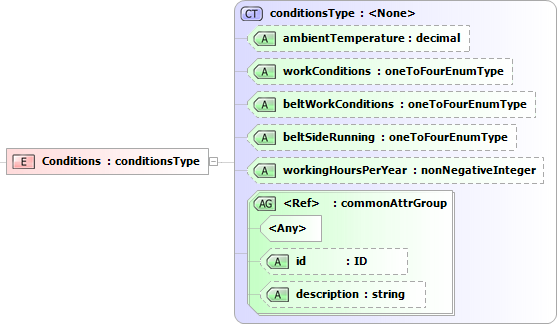
\includegraphics[width=0.6\textwidth]{png/liquid/Conditions}
  \caption{Definicja elementu Conditions}
  \label{fig:conditions-xsd}
\end{figure}

\noindent\textbf{Rodzice:} \texttt{BeltConveyor}

\noindent\textbf{Atrybuty:}
\begin{description}
\item[ambientTemperature] Temperatura otoczenia przenośnika - T [$^\circ$C]
\item[workConditions] Warunki pracy przenośnika: 1 - bardzo dobre, 2 - dobre,
  3 - przeciętne, 4 - ciężkie
\item[beltWorkConditions] Warunki eksploatacji taśmy: 1 - bardzo dobre,
  2 - dobre, 3 - przeciętne, 4 - ciężkie
\item[beltSideRunning] Zbieganie boczne taśmy: 1 - brak, 2 - małe, 3 - średnie,
  4 - duże
\item[workingHoursPerYear] Ilość godzin pracy przenośnika w ciągu roku
\end{description}


\subsection{Taśma <Belt>}\label{sec:Belt}
Taśma jest podstawowym elementem przenośnika. Taśma zamontowana na przenośniku
taśmowym jest najczęściej listą odcinków taśmy połączonym złączami.

\begin{figure}[H]
  \centering
  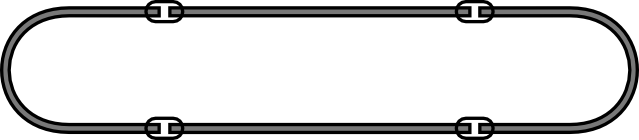
\includegraphics[width=0.6\textwidth]{png/tasma}
  \caption{Taśma przenośnikowa w uproszczeniu}
  \label{fig:belt-drw}
\end{figure}

Element {\tt Belt} jest jedynie elementem grupującym i nie ma swojej fizycznej
reprezentacji w konstrukcji przenośnika taśmowego. Element ten definiuje
strukturę, zgodnie z którą taśma przenośnikowa jest listą naprzemiennie
występujących elementów {\tt BeltSegment} oraz {\tt BeltSplice}, gdzie położenie
tych elementów w dokumencie odzwierciedla położenie odcinków i złącz w
rzeczywistej taśmie zamontowanej na przenośniku. Pierwsze złącze na liście łączy
ze sobą odcinek następujący bezpośrednio po nim oraz ostatni odcinek na liście,
w ten sposób domykając pętlę.

\begin{verbatim}
<Belt>
  <BeltSplice id="1" />
  <BeltSegment id="2" />
  <BeltSplice id="3" />
  <BeltSegment id="4" />
  <BeltSplice id="5" />
  <BeltSegment id="6" />
</Belt>
\end{verbatim}

W powyższym listingu odcinek taśmy 6 jest połączony złączem 5 z odcinkiem taśmy
4 oraz złączem 1 z odcinkiem taśmy 2. W najprostszym przypadku może być jedno
złącze i jeden odcinek.

\begin{figure}[H]
  \centering
  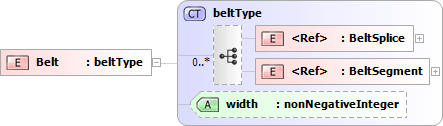
\includegraphics[width=0.6\textwidth]{png/belt_xsd2}
  \caption{Definicja elementu Belt}
  \label{fig:belt-xsd}
\end{figure}

\noindent\textbf{Rodzice:} \texttt{BeltConveyor}

\noindent\textbf{Atrybuty:}
\begin{description}
\item[width] Szerokość taśmy - B [mm]
\end{description}


\subsubsection{Odcinek taśmy <BeltSegment>}
Element {\tt BeltSegment} odzwierciedla fizycznie zamontowany na przenośniku
odcinek taśmy.  Atrybuty z grupy {\tt beltSegmentAttrGroup} mogą występować
bezpośrednio w elemencie {\tt BeltSegment} lub elemencie {\tt BeltSegmentType}
do którego można się odwoływać z elementu {\tt BeltSegment} za pomocą atrybutu
{\tt type}.  Cechą tej grupy atrybutów jest to, że mogą opisywać zarówno
instancję jak i typ odcinka taśmy. Atrybuty {\tt length} oraz {\tt cetificate}
mogą występować tylko w elemencie {\tt BeltSegment}.

\begin{figure}[H]
  \centering
  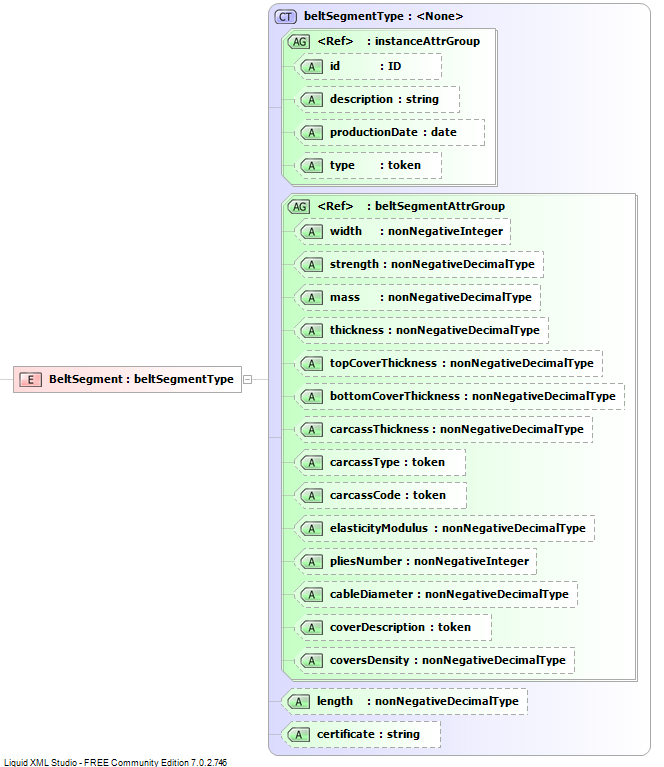
\includegraphics[width=0.6\textwidth]{png/liquid/BeltSegment}
  \caption{Definicja elementu BeltSegment}
  \label{fig:beltSegment-xsd}
\end{figure}

\noindent\textbf{Rodzice:} \texttt{Belt}

\noindent\textbf{Atrybuty:}
\begin{description}
\item[width] Szerokość odcinka taśmy [mm]
\item[strength] Nominalna wytrzymałość taśmy [kN/m]
\item[mass] Masa taśmy [kg/m]
\item[thickness] Grubość taśmy [mm]
\item[topCoverThickness] Grubość okładki górnej (nośnej) [mm]
\item[bottomCoverThickness] Grubość okładki dolnej (bieżnej) [mm]
\item[carcassThickness] Grubość rdzenia taśmy [mm]
\item[carcassType] Typ rdzenia taśmy (tkaninowa, z linkami stalowymi)
\item[carcassCode] Współczynnik rodzaju materiału rdzenia
\item[elasticityModulus] Moduł sprężystości taśmy - E [kN/m]
\item[pliesNumber] Liczba przekładek lub linek
\item[cableDiameter] Średnica linki [mm]
\item[coverDescription] Oznaczenie okładek
\item[coversDensity] Gęstość mieszanki okładkowej [kg/mm*m$^2$]
\item[length] Długość odcinka [m]
\item[certificate] Numer atestu
\end{description}


\subsubsection{Złącze <BeltSplice>}
Złącze w języku ConvML odnosi się do sąsiednich elementów na liście potomków
elementu {\tt Belt}.  W poprawnym dokumencie będą to zawsze elementy {\tt
  BeltSegment} reprezentujące odcinki taśmy.  Złącze w przeciwieństwie do
odcinka nie posiada parametru długości i jest rozpatrywane jako miejsce (punkt)
wykonania połączenia.

\begin{figure}[H]
  \centering
  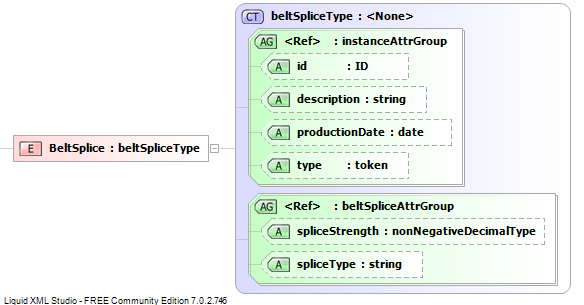
\includegraphics[width=0.6\textwidth]{png/liquid/BeltSplice}
  \caption{Definicja elementu BeltSplice}
  \label{fig:beltSplice-xsd}
\end{figure}

W przypadku złącza, standardowy atrybut {\tt productionDate} należy tłumaczyć
jako datę wykonania złącza.

\noindent\textbf{Rodzice:} \texttt{Belt}

\noindent\textbf{Atrybuty:}
\begin{description}
\item[spliceStrength] Wytrzymałość połączenia [\%]
\item[spliceType] Rodzaj złącza np: wulkanizowane, mechaniczne, klejone, inne.
\end{description}


\subsection{Stacja zwrotna <Tail>}
Stacja zwrotna jest elementem konstrukcyjnym przenośnika taśmowego w którym
taśma zmienia kierunek ruchu z trasy dolnej (powrotnej) na trasę górną (nośną).
Zmiana kierunku odbywa się na bębnie zwrotnym, który jest pierwszym podelementem
elementu {\tt Tail} w strukturze.  Elementy {\tt Carry} oraz {\tt Return}
odpowiadają trasie nośnej oraz trasie powrotnej i są opisane w rozdziale
dotyczącym segmentów trasy.

\begin{figure}[H]
  \centering
  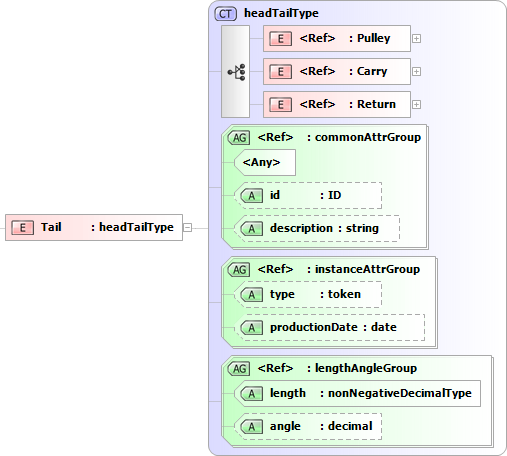
\includegraphics[width=0.6\textwidth]{png/liquid/Tail}
  \caption{Definicja elementu Tail}
  \label{fig:tail-xsd}
\end{figure}

\noindent\textbf{Rodzice:} \texttt{BeltConveyor}


\subsection{Stacja czołowa <Head>}
Stacja czołowa pomimo innej nazwy elementu w stosunku do stacji zwrotnej posiada
dokładnie taką samą definicję podelementów.  Zmienia się jedynie interpretacja
elementu {\tt Pulley}, który w tym przypadku odpowiada bębnowi czołowemu i obywa
się na nim zmiana kierunku taśmy z trasy nośnej na trasę powrotną.

\begin{figure}[H]
  \centering
  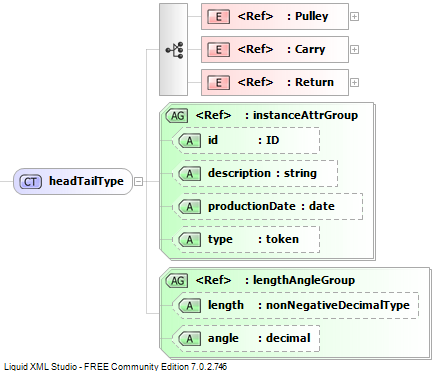
\includegraphics[width=0.6\textwidth]{png/liquid/headTailType}
  \caption{Definicja typu elementu Head}
  \label{fig:headTailType-xsd}
\end{figure}

\noindent\textbf{Rodzice:} \texttt{BeltConveyor}


\subsection{Bęben <Pulley>}
Element {\tt Pulley} reprezentuje bęben w strukturze przenośnika.  Poza bębnami
zwrotnym oraz czołowym, które posiadają określone miejsca w strukturze, można
umieścić dodatkowe bębny w strukturze przenośnika jako podelementy elementów
{\tt Carry} (górna trasa) oraz {\tt Return} (dolna trasa).

Ze względu na funkcję rozróżnia się w przenośnikach bębny napędowe; napinające,
zapewniające niezbędne napięcie taśmy; odchylające lub odginające, zwiększające
kąt opasania taśmy.

W języku ConvML bębny wszystkich rodzajów oznacza się tym samym elementem {\tt
  Pulley}.  O ich funkcji decydują elementy zawarte wewnątrz elementu {\tt
  Pulley}. Przy braku tych elementów bęben pełni funkcję odchylającą.  Przy
obecności jednego lub dwóch zestawów napędowych ({\tt DriveUnit}) staje się
bębnem napędowym.  Analogicznie obecność zestawu napinającego ({\tt
  TakeUpSystem}) informuje o funkcji napinającej bębna.

\begin{figure}[H]
  \centering
  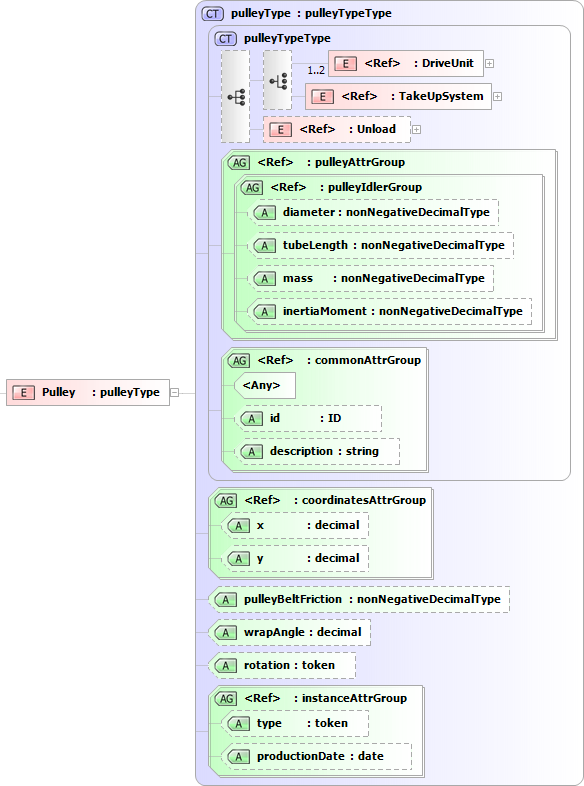
\includegraphics[width=0.6\textwidth]{png/liquid/Pulley}
  \caption{Definicja elementu Pulley}
  \label{fig:pulley-xsd}
\end{figure}

\noindent\textbf{Rodzice:} \texttt{Carry, Return, TTDrive}

\noindent\textbf{Atrybuty:}
\begin{description}
\item[diameter] Średnica [m]
\item[pulleyBeltFriction] Współczynnik tarcia między taśmą a bębnem napędowym
\item[wrapAngle] Kąt opasania taśmą - $\alpha$ [$^\circ$]
\item[x] Położenie osi bębna względem elementu nadrzędnego [m]
\item[y] Położenie osi bębna względem elementu nadrzędnego [m]
\item[rotation] Rotacja bębna: cw - zgodnie z ruchem wskazówek zegara;
	ccw - przeciwnie względem ruchu wskazówek zegara.
\item[mass] Masa [kg]
\item[inertiaMoment] Moment bezwładności - I [kgm$^2$]
\end{description}


\subsection{Trasa <Route>}\label{sec:Route}
Trasa jest elementem grupującym odcinki trasy. Aby obliczyć całkowitą długość
przenośnika, wysokość podnoszenia oraz pozostałe parametry geometryczna należy
wziąć pod uwagę wszystkie odcinki trasy oraz stację czołową i zwrotną.  Element
{\tt Route} nie posiada atrybutów.

\begin{figure}
  \centering
  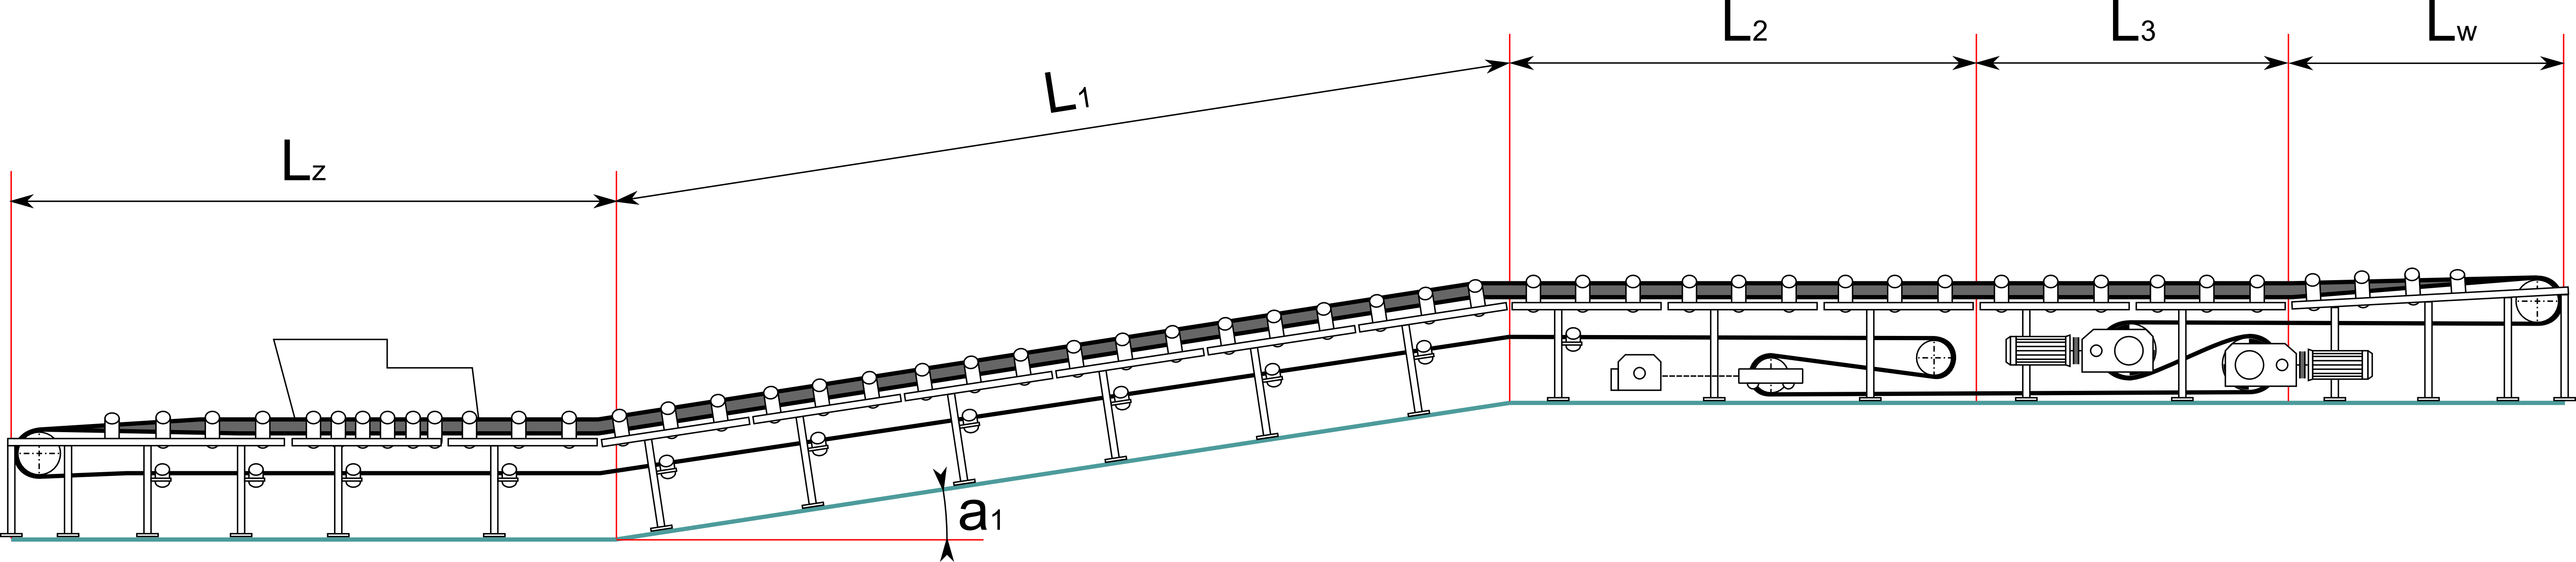
\includegraphics[width=\textwidth]{png/belt_conveyor2_drw}
  \caption{Odcinki trasy przenośnika taśmowego}
  \label{fig:beltConveyor2-drw}
\end{figure}

\begin{figure}[H]
  \centering
  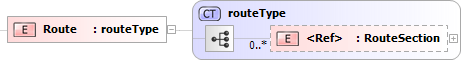
\includegraphics[width=0.6\textwidth]{png/liquid/Route}
  \caption{Definicja elementu Route}
  \label{fig:route-xsd}
\end{figure}

\noindent\textbf{Rodzice:} \texttt{BeltConveyor}


\subsubsection{Odcinek trasy <RouteSection>}
Odcinek trasy jest elementem logicznego podziału trasy przenośnika na elementy o
różnej długości oraz nachyleniu. Podział na odcinki umożliwia zapis podstawowych
parametrów geometrycznych przenośnika.

Odcinek składa się z listy segmentów. Lokalizacja segmentu zależy od jego
pozycji na liście oraz sumarycznej długości segmentów poprzedzających. Jeśli
odcinek jest łukowy, segmenty z których się składa są "wpisane" w ten łuk co
powoduje, że nie ma konieczności określania kąta nachylenia dla każdego segmentu
z osobna.

Sumaryczna długość segmentów nie może przekraczać długości odcinka trasy do
którego należą segmenty.

Jeśli nie ma konieczności ewidencjonowania segmentów trasy możliwe jest
wskazanie jedynie typu segmentów z jakich składa się odcinek. Służy do tego
atrybut {\tt segmentType}. Ograniczeniem tego rozwiązania jest fakt, że w takim
przypadku odcinek może się składać jedynie z segmentów tego samego typu.

\begin{figure}[H]
  \centering
  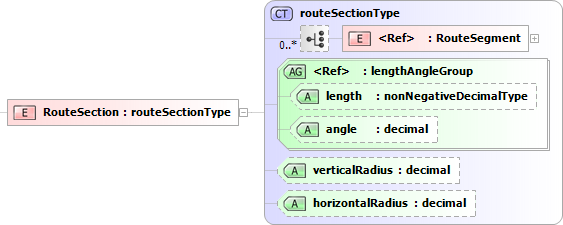
\includegraphics[width=0.6\textwidth]{png/liquid/RouteSection}
  \caption{Definicja elementu RouteSection}
  \label{fig:routeSection-xsd}
\end{figure}

\noindent\textbf{Rodzice:} \texttt{Route}

\noindent\textbf{Atrybuty:}
\begin{description}
\item[length] Długość elementu [m]
\item[angle] Kąt nachylenia elementu [$^\circ$]
\item[verticalRadius] Promień łuku wertykalnego [m]
\item[horizontalRadius] Promień łuku horyzontalnego [m]
\item[segmentType] Typ segmentów z których składa się odcinek, w przypadaku w
  którym segmenty nie są jawnie zdefiniowane jako podelementy
\end{description}


\subsubsection{Segment trasy <RouteSegment>}
Segment trasy jest fizycznym elementem konstrukcyjnym który umożliwia montaż
podzespołów współpracujących z taśmą poruszającą się na trasie powrotnej lub
nośnej.

Do określenia czy elementy zamontowane na segmencie są częścią trasy nośnej, czy
trasy powrotnej, służą elementy {\tt Carry} oraz {\tt Return}.

\begin{figure}[H]
  \centering
  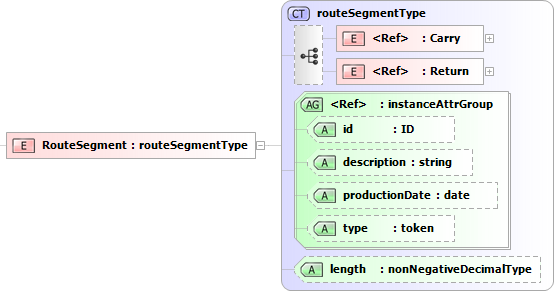
\includegraphics[width=0.6\textwidth]{png/liquid/RouteSegment}
  \caption{Definicja elementu RouteSegment}
  \label{fig:routeSegment-xsd}
\end{figure}

\noindent\textbf{Rodzice:} \texttt{RouteSection}

\noindent\textbf{Atrybuty:}
\begin{description}
\item[length] Długość elementu [m]
\end{description}


\subsubsection{Górna trasa <Carry>}
Element Carry grupuje obiekty współpracujące z taśmą poruszającą się po trasie
nośnej.

\begin{figure}[H]
  \centering
  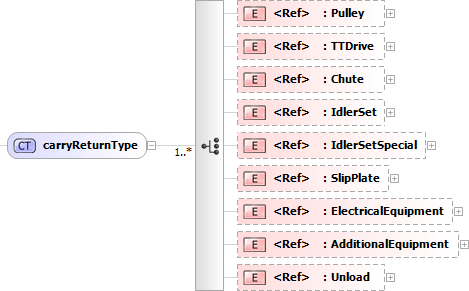
\includegraphics[width=0.6\textwidth]{png/liquid/carryReturnType}
  \caption{Definicja typu elementu Carry}
  \label{fig:carryReturnType-xsd}
\end{figure}

\noindent\textbf{Rodzice:} \texttt{RouteSegment, Head, Tail}


\subsubsection{Dolna trasa <Return>}
Element {\tt Return} grupuje obiekty współpracujące z taśmą poruszającą się po
trasie powrotnej.  Element ten modyfikuje układ współrzędnych dla swoich
podelementów.  Oś x jest zwrócona w przeciwnym kierunku względem elementu
nadrzędnego i jej zwrot jest zgodny z kierunkiem biegu taśmy.  Środek układu
współrzędnych jest przesunięty.  Zakładając że $(x_0, y_0)$ to środek układu
współrzędnych elementu nadrzędnego ({\tt RouteSegment, Head, Tail}) to nowy
środek układu znajduje się w punkcie $(x_0 + {length}, y_0)$, gdzie ${length}$
jest atrybutem długości elementu nadrzędnego.

\begin{figure}[H]
  \centering
  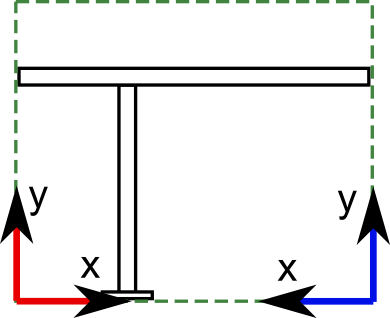
\includegraphics[width=0.4\textwidth]{png/carryReturn_drw}
  \caption{Układy współrzędnych elementów Carry (czerwony) oraz
elementu Return (niebieski)}
  \label{fig:carryReturn-drw}
\end{figure}

\noindent\textbf{Rodzice:} \texttt{RouteSegment, Head, Tail}

\subsection{Zespół napędowy <DriveUnit>}
Element grupujący urządzenia wchodzące w skład zespołu napędowego. Może
występować jedynie jako podelement elementu {\tt Pulley} (Bębna).

\begin{figure}[H]
  \centering
  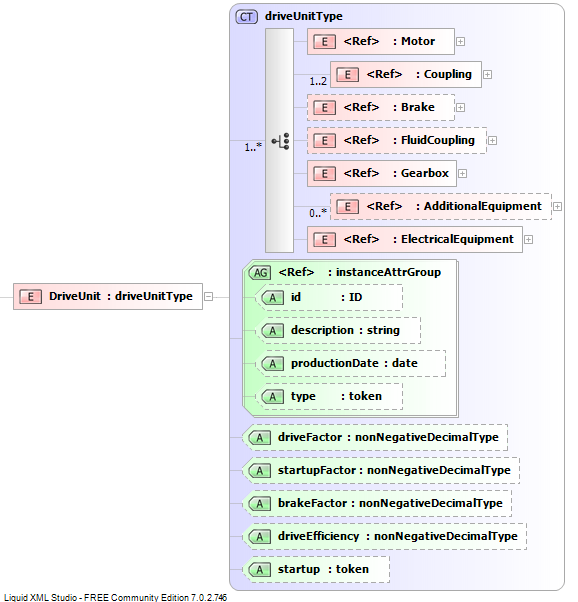
\includegraphics[width=0.6\textwidth]{png/liquid/DriveUnit}
  \caption{Definicja elementu DriveUnit}
  \label{fig:driveUnit-xsd}
\end{figure}

\noindent\textbf{Rodzice:} \texttt{Pulley}

\noindent\textbf{Atrybuty:}
\begin{description}
\item[dynamicSurplusFactor] Współczynnik nadwyżki dynamicznej $K_D = M_R/M_U$,
  gdzie $M_R$ - moment rozruchowy, $M_U$ - moment ustalony
\item[brakeFactor] Stosunek momentu hamowania do nominalnego momentu napędu $K_H
  = M_H/M_N$, gdzie $M_H$ - moment hamowania, $M_N$ - moment nominalny
\item[driveEfficiency] Sprawność napędu - $\eta$
\item[startupControlSystem] Urządzenie rozruchowe
\end{description}

\subsubsection{Silnik <Motor>}

\begin{figure}[H]
  \centering
  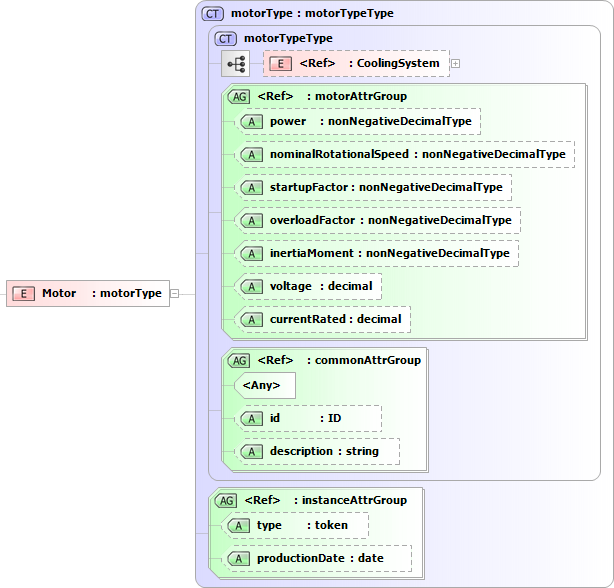
\includegraphics[width=0.6\textwidth]{png/liquid/Motor}
  \caption{Definicja elementu Motor}
  \label{fig:motor-xsd}
\end{figure}

\noindent\textbf{Rodzice:} \texttt{DriveUnit}

\noindent\textbf{Atrybuty:}
\begin{description}
\item[power] Moc silnika [kW]
\item[nominalRotationalSpeed] Nominalna prędkość obrotowa [1/min]
\item[startupFactor] Współczynnik rozruchowy $K_R = M_R/M_N$,
	gdzie $M_R$ - moment rozruchowy, $M_N$ - moment nominalny
\item[overladFactor] Współczynnik przeciążalności napędu $K_O = M_{Max}/M_N$,
	gdzie $M_{Max}$ - moment maksymalny, $M_N$ - moment nominalny
\item[inertiaMoment] Moment bezwładności [kgm$^2$]
\item[voltage] Napięcie zasilania
\item[currentRated] Prąd znamionowy silnika
\end{description}

\subsubsection{Sprzęgło podatne <Coupling>}

\begin{figure}[H]
  \centering
  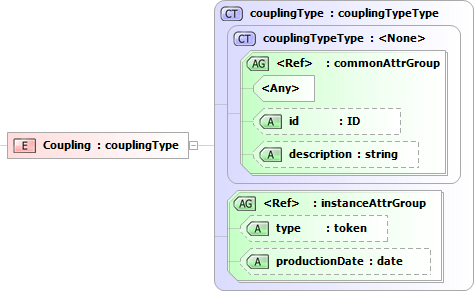
\includegraphics[width=0.6\textwidth]{png/liquid/Coupling}
  \caption{Definicja elementu Coupling}
  \label{fig:coupling-xsd}
\end{figure}

\noindent\textbf{Rodzice:} \texttt{DriveUnit}

\subsubsection{Sprzęgło hydrodynamiczne <FluidCoupling>}

\begin{figure}[H]
  \centering
  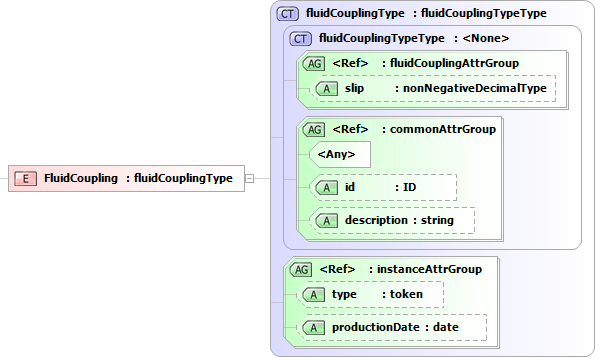
\includegraphics[width=0.6\textwidth]{png/liquid/FluidCoupling}
  \caption{Definicja elementu FluidCoupling}
  \label{fig:fluidCoupling-xsd}
\end{figure}

\noindent\textbf{Rodzice:} \texttt{DriveUnit}

\noindent\textbf{Atrybuty:}
\begin{description}
\item[slip] Poślizg sprzęgła
\end{description}


\subsubsection{Układ hamulcowy <Break>}

\begin{figure}[H]
  \centering
  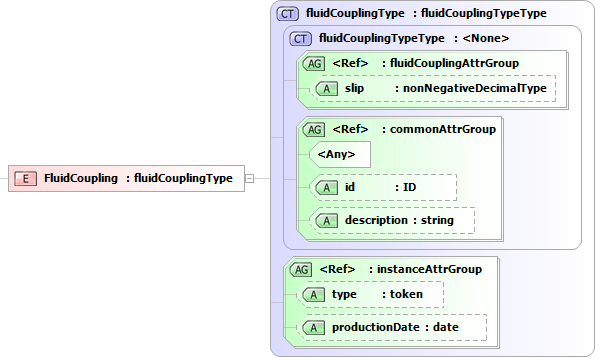
\includegraphics[width=0.6\textwidth]{png/liquid/FluidCoupling}
  \caption{Definicja elementu Break}
  \label{fig:break-xsd}
\end{figure}

\noindent\textbf{Rodzice:} \texttt{DriveUnit}

\subsubsection{Przekładnia <Gearbox>}

\begin{figure}[H]
  \centering
  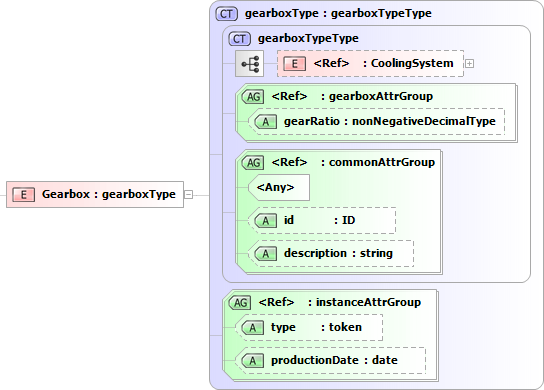
\includegraphics[width=0.6\textwidth]{png/liquid/Gearbox}
  \caption{Definicja elementu Gearbox}
  \label{fig:gearbox-xsd}
\end{figure}

\noindent\textbf{Rodzice:} \texttt{DriveUnit}

\noindent\textbf{Atrybuty:}
\begin{description}
\item[gearRatio] Przełożenie przekładni
\end{description}


\subsection{Zespół napinający <TakeUpSystem>}

\begin{figure}[H]
  \centering
  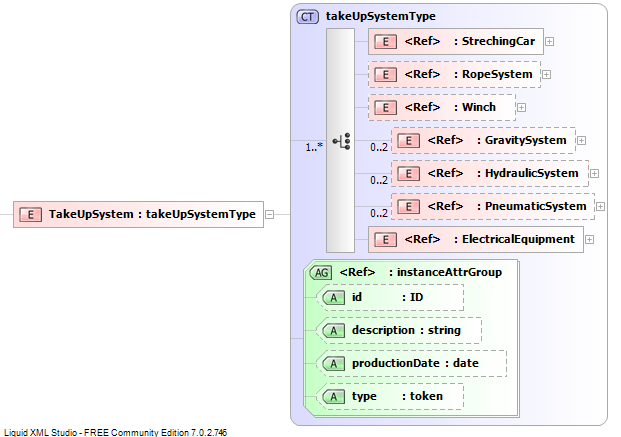
\includegraphics[width=0.6\textwidth]{png/liquid/TakeUpSystem}
  \caption{Definicja elementu TakeUpSystem}
  \label{fig:takeUpSystem-xsd}
\end{figure}

\noindent\textbf{Rodzice:} \texttt{Pulley}

\subsubsection{Wózek napinający <StrechingCar>}

\begin{figure}[H]
  \centering
  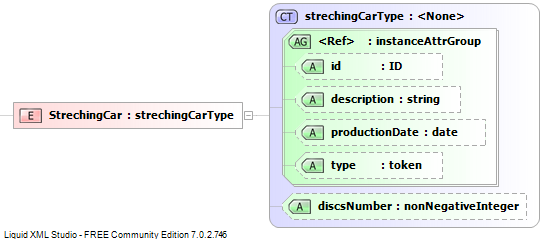
\includegraphics[width=0.6\textwidth]{png/liquid/StrechingCar}
  \caption{Definicja elementu StrechingCar}
  \label{fig:strechingCar-xsd}
\end{figure}

\noindent\textbf{Rodzice:} \texttt{TakeUpSystem}

\noindent\textbf{Atrybuty:}
\begin{description}
\item[numberOfDiscs] Liczba krążków
\end{description}


\subsubsection{Układ zlinowania <RopeSystem>}

\begin{figure}[H]
  \centering
  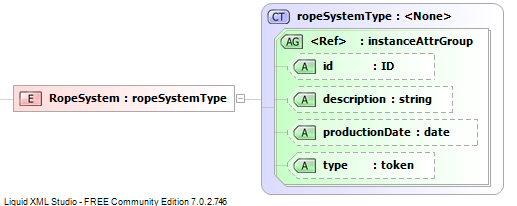
\includegraphics[width=0.6\textwidth]{png/liquid/RopeSystem}
  \caption{Definicja elementu RopeSystem}
  \label{fig:ropeSystem-xsd}
\end{figure}

\noindent\textbf{Rodzice:} \texttt{TakeUpSystem}


\subsubsection{Obciążnik <Counterweight>}

\noindent\textbf{Rodzice:} \texttt{GravitySystem}

\noindent\textbf{Atrybuty:}
\begin{description}
\item[numberOfDiscs] Liczba krążków
\item[mass] Masa obciążnika
\end{description}


\subsubsection{Wciągarka <Winch>}

\noindent\textbf{Rodzice:} \texttt{TakeUpSystem}

\noindent\textbf{Atrybuty:}
\begin{description}
\item[takeUpTension] Siła naciągu [kN]
\end{description}


\subsubsection{Układ grawitacyjny <GravitySystem>}

\noindent\textbf{Rodzice:} \texttt{TakeUpSystem}


\subsubsection{Układ hydrauliczny <HydraulicSystem>}

\noindent\textbf{Rodzice:} \texttt{TakeUpSystem}


\subsubsection{Układ pneumatyczny <PneumaticSystem>}

\noindent\textbf{Rodzice:} \texttt{TakeUpSystem}

\subsection{Kosz zasypowy <Chute>}
Kosz zasypowy jako element trasy wyznacza miejsce załadunku materiału na
przenośnik taśmowy.

\begin{figure}[H]
  \centering
  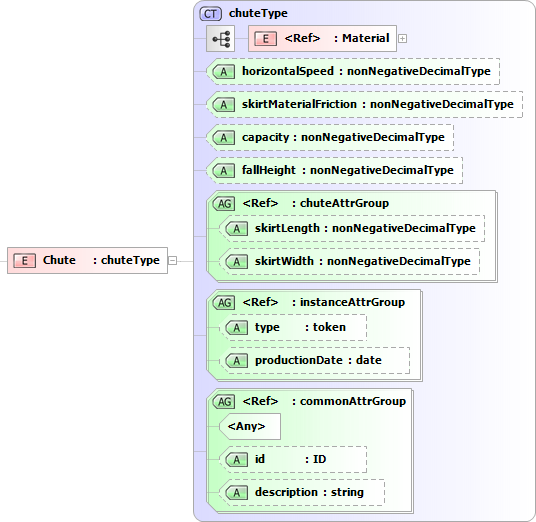
\includegraphics[width=0.6\textwidth]{png/liquid/Chute}
  \caption{Definicja elementu Chute}
  \label{fig:chute-xsd}
\end{figure}

\noindent\textbf{Rodzice:} \texttt{Carry, Return}

\noindent\textbf{Atrybuty:}
\begin{description}
\item[horizontalSpeed] Składowa prędkości taśmy [m/s]
\item[skirtMaterialFriction] Współczynnik tarcia pomiędzy urobkiem a
  ograniczeniami bocznymi
\item[capacity] Wydajność punktu załadowczego [t/h]
\item[fallHeight] Wysokość spadku materiału na taśmę [mm]
\item[skirtLength] Długość ograniczeń bocznych [m]
\item[skirtWidth] Szerokość ograniczeń bocznych [m]
\end{description}


\subsubsection{Materiał <Material>}
Element opisujący właściwości materiału podawanego na kosz zasypowy.

\begin{figure}[H]
  \centering
  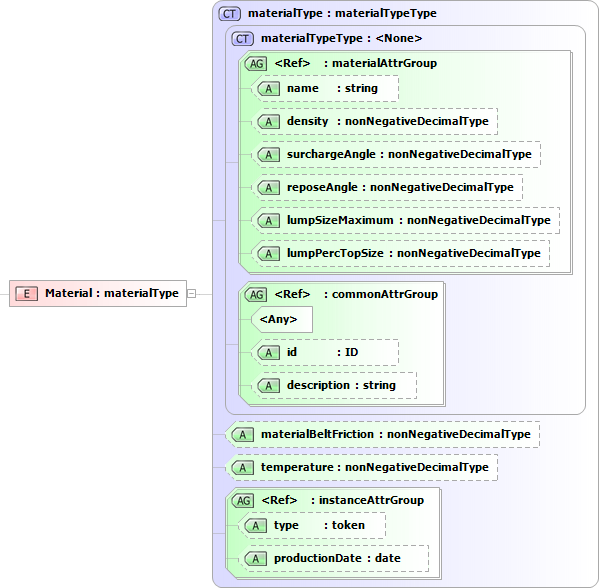
\includegraphics[width=0.6\textwidth]{png/liquid/Material}
  \caption{Definicja elementu Material}
  \label{fig:material-xsd}
\end{figure}

\noindent\textbf{Rodzice:} \texttt{Chute}

\noindent\textbf{Atrybuty:}
\begin{description}
\item[name] Nazwa materiału
\item[density] Gęstość nasypowa materiału transportowanego - $\gamma$ [$kg/m^3$]
\item[surchargeAngle] Kąt usypu materiału na taśmie - $\rho$ [$^\circ$]
\item[reposeAngle] Kąt tarcia wewnętrznego [$^\circ$]
\item[lumpSizeMaximum] Maksymalny wymiar brył [mm]
\item[lumpPercTopSize] Procentowy udział brył [\%]
\item[materialBeltFriction] Współczynnik tarcia urobek-taśma
\item[temperature] Temperatura materiału [$^\circ$C]
\end{description}


\subsection{Rozładunek <Unload>}
Wyznacze miejsce rozładunku przenośnika. Jeśli występuje pod elementem {\tt Pulley}
oznacza rozładuek przez bęben.  Element {\tt Unload} może również występować w
dowolnym miejscu trasy co jest utożsamiane z urządzeniem typu pług rozładowczy.

\noindent\textbf{Rodzice:} \texttt{Pulley, Carry, Return}


\subsection{Elementy trasy}

\subsubsection{Pojedynczy krążnik <Idler>}
Podstawowym zadaniem krążników jest właściwe ukształtowanie, podtrzymywanie i
ochrona taśmy, a także zmniejszenie oporów ruchu przenośnika oraz właściwe
podtrzymywanie transportowanego nosiwa.  Opory tarcia krążnika wpływają na siły
napięcia taśmy i na zapotrzebowanie mocy napędu \cite{Antoniak2005}.  W języku
ConvML pojedynczemu krążnikowi odpowiada element {\tt Idler}. Krążniki pracują w
zestawach ({\tt IdlerSet}).

\begin{figure}[H]
  \centering
  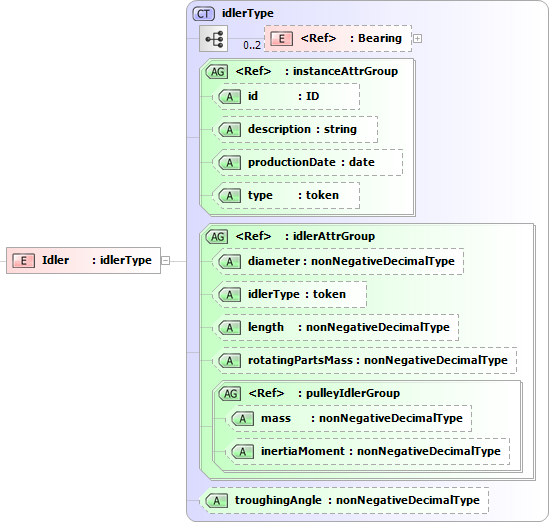
\includegraphics[width=0.6\textwidth]{png/liquid/Idler}
  \caption{Definicja elementu Idler}
  \label{fig:idler-xsd}
\end{figure}

\noindent\textbf{Rodzice:} \texttt{IdlerSet, IdlerSetSpecial}

\noindent\textbf{Atrybuty:}
\begin{description}
\item[diameter] Średnica krążnika [mm]
\item[idlerType] Typ krążnika: 1 - z pierścieniami, 2 - gładki
\item[length] Długość płaszcza krążnika [mm]
\item[troughingAngle] Kąt nachylenia krążników bocznych - $\beta$ [$^\circ$]
\item[rotatingPartsMass] Masa części obrotowych krążnika [kg]
\item[mass] Masa [kg]
\item[inertiaMoment] Moment bezwładności - I [$kg*m^2$]
\end{description}


\subsubsection{Zestaw krążnikowy <IdlesSet>}
Krążniki montuje się na trasie przenośnika (górnej lub dolnej) w postaci
zestawów.  W przypadku braku współrzędnej X, zestawy są rozmieszczane w równej
odległości na długości segmentu trasy ({\tt RouteSegment}).

\begin{figure}[H]
  \centering
  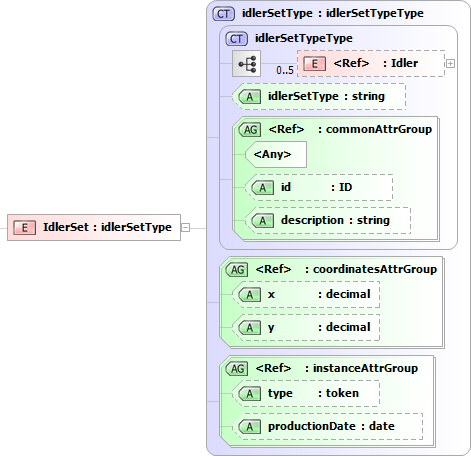
\includegraphics[width=0.6\textwidth]{png/liquid/IdlerSet}
  \caption{Definicja elementu IdlerSet}
  \label{fig:idlerSet-xsd}
\end{figure}

\noindent\textbf{Rodzice:} \texttt{Carry, Return}

\noindent\textbf{Atrybuty:}
\begin{description}
\item[x] Położenie osi krążnika środkowego względem elementu nadrzędnego [m]
\item[y] Położenie osi krążnika środkowego względem elementu nadrzędnego [m]
\end{description}


\subsubsection{Zestaw specjalny <IdlesSetSpecial>}
\noindent\textbf{Rodzice:} \texttt{Carry, Return}

\subsubsection{Płyta ślizgowa <SlipPlate>}
\noindent\textbf{Rodzice:} \texttt{Carry, Return}

\subsubsection{Napęd typu taśma-taśma <TTDrive>}
Napęd pośredni taśma-taśma jest wyposażony w bęben napędowy, napinający oraz
trasę.  Napęd ten jest usytuowany na trasie przenośnika głównego wewnątrz jego
obrysu.

\begin{figure}[H]
  \centering
  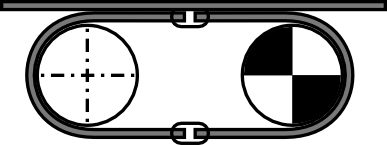
\includegraphics[width=0.4\textwidth]{png/naped_tt}
  \caption{Napęd typu taśma-taśma}
  \label{fig:ttDrive-drw}
\end{figure}

\begin{figure}[H]
  \centering
  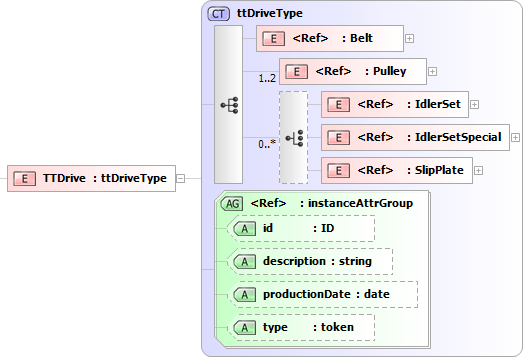
\includegraphics[width=0.6\textwidth]{png/liquid/TTDrive}
  \caption{Definicja elementu TTDrive}
  \label{fig:ttDrive-xsd}
\end{figure}

\noindent\textbf{Rodzice:} \texttt{Carry, Return}


\subsection{Wyposażenie elektryczne przenośnika <ConvElectricalEquipment>}
Wyposażenie elektryczne współpracujące z przenośnikiem taśmowym jako całością.

\noindent\textbf{Rodzice:} \texttt{BeltConveyor}


\subsubsection{Układ sterowania przenośnikiem <ControlSystem>}
\noindent\textbf{Rodzice:} \texttt{ConvElectricalEquipment}

\subsubsection{System wyłączenia awaryjnego <EmergencySystem>}
\noindent\textbf{Rodzice:} \texttt{ConvElectricalEquipment}

\subsubsection{System łączności i sygnalizacji <SignalSystem>}
\noindent\textbf{Rodzice:} \texttt{ConvElectricalEquipment}

\subsubsection{Instalacja przeciwpożarowa <FireSystem>}
\noindent\textbf{Rodzice:} \texttt{ConvElectricalEquipment}

\subsection{Pozostałe}

\subsubsection{Układ chłodzenia <CoolingSystem>}
\noindent\textbf{Rodzice:} \texttt{Motor, Gearbox}

\subsubsection{Urządzenie czyszczące <CleaningDevice>}


\subsubsection{Wyposażenie elektryczne urządzenia <ElectricalEquipment>}
\noindent\textbf{Rodzice:} \texttt{Carry, Return, TakeUpSystem, DriveUnit}


\subsubsection{Urządzenie dodatkowe <AdditionalEquipment>}
\noindent\textbf{Rodzice:} \texttt{Carry, Return, DriveUnit}


\section{Typy <Types>}\label{sec:Types}
Do formatu ConvML w wersji 1.2 wprowadzono pojęcie typu w celu uniknięcia
niepotrzebnych powtórzeń.  Typ w sensie rozumianym przez ConvML jest zbiorem
wartości atrybutów, które mogą być współdzielone przez wiele instancji tego
samego elementu.  Typy definiuje się wewnątrz elementu {\tt Types}, a ich nazwa
tworzona jest poprzez dodanie do nazwy elementu sufiksu {\tt Type}. Każdy Typ
musi posiadać unikalny atrybut {\tt typeId}.


\subsection{Typy płaskie}
W najprostszym przypadku instancja elementu {\tt BeltSegment} dziedziczy
wartości atrybutów zdefiniowanych w elemencie {\tt BeltSegmentType} jeśli
wartość atrybutu {\tt type} zgadza się z wartością atrybutu {\tt typeId}.  Nie
jest dopuszczalne przedefiniowanie atrybutów zdefiniowanych w typie.

\begin{verbatim}
<Types>
  <BeltSegmentType typeId="GTP-1200/t"
                   bottomCoverThickness="2"
                   carcassType="tekstylny"
                   coverDescription="trudnopalna"
                   elasticityModulus="2000"
                   manufacturer="Wolbrom"
                   pliesNumber="3"
                   topCoverThickness="4"
                   width="1200"/>
</Types>
\end{verbatim}

\begin{verbatim}
<Belt>
  <BeltSplice/>
  <BeltSegment type="GTP-1200/t"
               length="100"
               productionDate="2005-04-11"
               certificate="1257"/>
  <BeltSplice/>
  <BeltSegment type="GTP-1200/t"
               length="100"
               productionDate="2005-07-15"
               certificate="1258"/>
</Belt>
\end{verbatim}


\subsection{Typy złożone}
Typy mogą posiadać zdefiniowane podelementy.  W takim przypadku w elemencie
odwołującym się do typu nie może już być podelementów.

\begin{verbatim}
<IdlerType typeId="133" />
<IdlerSetType typeId="A">
  <Idler type="133"/>
  <Idler type="133"/>
  <Idler type="133"/>
</IdlerSetType>
\end{verbatim}

\begin{verbatim}
<IdlerSet type="A"/>
\end{verbatim}

Jeśli element może mieć podelementy, a typ do którego się odwołuje nie posiada
podelementów, to taki element może posiadać podelementy.

\begin{verbatim}
<IdlerSetType typeId="B"/>
\end{verbatim}

\begin{verbatim}
<IdlerSet type="B">
  <Idler type="133"/>
  <Idler type="133"/>
  <Idler type="133"/>
<IdlerSet/>
\end{verbatim}

\section{Metadane dokumentu <Meta>}
Element {\tt Meta} umożliwia zapisanie dodatkowych informacji o dokumencie.
Jest jedynym elementem w którego strukturze występują węzły tekstowe.

\noindent\textbf{Definicje podelementów:}
\begin{description}
\item[Generator] Program który utworzył dokument
\item[Title] Opcjonalny tytuł dokumentu
\item[Description] Opcjonalny opis dokumentu
\item[Creator] Użytkownik który utworzył dokument
\item[CreationDate] Data utworzenia dokumentu
\item[ModifiedBy] Użytkownik który ostatnio modyfikował dokument
\item[ModifiedDate] Data ostatniej modyfikacji
\item[Language] Kod języka w którym utworzono dokument.
	Atrybut link wskazuje plik z tłumaczeniami.
\item[UnitSystem] System jednostek. Atrybut link wskazuje plik z definicjami jednostek. 
\end{description}

\section{Grupy atrybutów}
Atrybuty wspólne dla różnych elementów zdefiniowano w grupach do których można
się odwoływać w dokumencie XML Schema opisującym ConvML'a.

\subsection{commonAttrGroup}
Atrybuty mogące wystąpić w każdym elemencie dokumentu ConvML.

\begin{description}
\item[id] Numer identyfikacyjny elementu. Musi być unikalny w skali dokumentu.
\item[description] Dowolny opis elementu
\end{description}

\subsection{instanceAttrGroup}
Atrybutu mogące wystąpić w elementach, które mogą być typizowane.

\begin{description}
\item[type] Identyfikator typu do którego element się odwołuje
\item[productionDate] Data produkcji 
\end{description}

\subsection{typeAttrGroup}
Atrybuty występujące w elementach opisujących Typ obiektu wchodzącego w skład
przenośnika.  Są to podelementy elementu {\tt Types}.

\begin{description}
\item[typeId] Identyfikator typu. Musi być unikalny.
\item[typeName] Nazwa handlowa
\item[typeDescription] Opis typu. Ten opis nie zostanie nadpisany przez atrybut
  description w instancji odwołującej się do typu.
\item[manufacturer] Producent elementów należących do opisywanego typu. 
\end{description}

\subsection{lengthAngleGroup}
Atrybuty elementów mających długość i kąt nachylenia. Wspólne dla stacji
zwrotnej, stacji czołowej oraz odcinków trasy.

\begin{description}
\item[length] Długość elementu [m]
\item[angle] Kąt nachylenia elementu w przedziale <-90, 90> [$^\circ$] 
\end{description}

\subsection{takeUpTensionGroup}
Atrybuty wspólne dla mechanizmów napinających.

\begin{description}
\item[takUpTension] Siła napinająca [kN]
\end{description}

\subsection{pulleyIdlerGroup}
Atrybuty wspólne bębnów i krążników.

\begin{description}
\item[mass] Masa [kg]
\item[inertiaMoment] Moment bezwładności - I [$kg*m^2$]
\end{description}

\subsection{coordinatesAttrGroup}
Atrybuty wspólne dla urządzeń których położenie jest opisane współrzędnymi.

\begin{description}
\item[x] Położenie punktu $x_0$ względem elementu nadrzędnego [m]
\item[y] Położenie punktu $y_0$ względem elementu nadrzędnego [m]
\end{description}

\section{Rozszerzenia XSD}
Typy danych nie występujące w XML Schema.

\subsection{nonNegativeDecimalType}
Typy {\tt xs:decimal} o wartościach nieujemnych.

\begin{verbatim}
<xs:simpleType name="nonNegativeDecimalType">
  <xs:restriction base="xs:decimal">
    <xs:minInclusive value="0" />
  </xs:restriction>
</xs:simpleType>
\end{verbatim}

\subsection{oneToFourEnumType}
Wyliczenie o bazie znakowej.

\begin{verbatim}
<xs:simpleType name="oneToFourEnumType">
  <xs:restriction base="xs:token">
    <xs:enumeration value="1" />
    <xs:enumeration value="2" />
    <xs:enumeration value="3" />
    <xs:enumeration value="4" />
  </xs:restriction>
</xs:simpleType>
\end{verbatim}


\section{Szablony}
Podstawowe dokumenty ConvML.

\subsection{BeltConvEditor 2.0}
Poniższy dokument jest wykorzystywany jako baza do nowego projektu
przenośnika taśmowego w programie BeltConvEditor.

\begin{verbatim}
<?xml version="1.0" encoding="utf-8"?>
<ConvML version="1.2"
        xmlns="http://www.entertech.com.pl/convml">
  <BeltConveyor>
    <Conditions/>
    <Belt>
      <BeltSplice/>
      <BeltSegment/>
    </Belt>
    <Tail length="50" angle="5">
      <Pulley y="2" diameter="1"/>
      <Carry>
        <Chute>
          <Material/>
        </Chute>
      </Carry>
      <Return/>
    </Tail>
    <Route>
      <RouteSection length="50">
        <RouteSegment>
          <Carry/>
          <Return/>
        </RouteSegment>
      </RouteSection>
    </Route>
    <Head length="50" angle="5">
      <Pulley y="2" diameter="1">
        <DriveUnit>
          <Motor/>
          <Coupling/>
          <Gearbox/>
          <ElectricalEquipment/>
        </DriveUnit>
      </Pulley>
      <Carry/>
      <Return/>
    </Head>
    <ConvElectricalEquipment>
      <ControlSystem/>
      <EmergencySystem/>
      <SignalSystem/>
      <FireSystem/>
    </ConvElectricalEquipment>
  </BeltConveyor>
</ConvML>
\end{verbatim}

\bibliographystyle{abbrv}
\bibliography{all}
\end{document}
